\documentclass[
  11pt,
  letterpaper,
   addpoints,
   answers
  ]{exam}

\usepackage{../exercise-preamble}
\usepackage{float}

\begin{document}

\noindent
\begin{minipage}{0.47\textwidth}

\includegraphics[width=\textwidth]{../fcfm_die}
\end{minipage}
\begin{minipage}{0.53\textwidth}
\begin{center}
\large\textbf{Análisis de Sistemas Dinámicos y Estimación} (EL3204-1) \\
\large\textbf{Clase auxiliar 2} \\
\normalsize Prof.~ Marcos Orchard - Sebastián Espinosa.\\
\normalsize Prof.~Aux.~Erik Sáez
\end{center}
\end{minipage}

\vspace{0.5cm}
\noindent
\vspace{.85cm}

\begin{questions}
    %%%%%%%%%%%%%%%%%%%%%%%%%%%
    \question Considere el siguiente circuito eléctrico, donde \(\alpha(t)i_2(t)\) corresponde al valor de la resistencia eléctrica de un potenciómetro, cuyo valor depende tanto de \(\alpha(t)\) como de la corriente que circula por el condensador, y \(v_{out}(t)\) (voltaje en el condensador) se mide con un voltímetro.
\begin{figure}[ht]
        \centering
        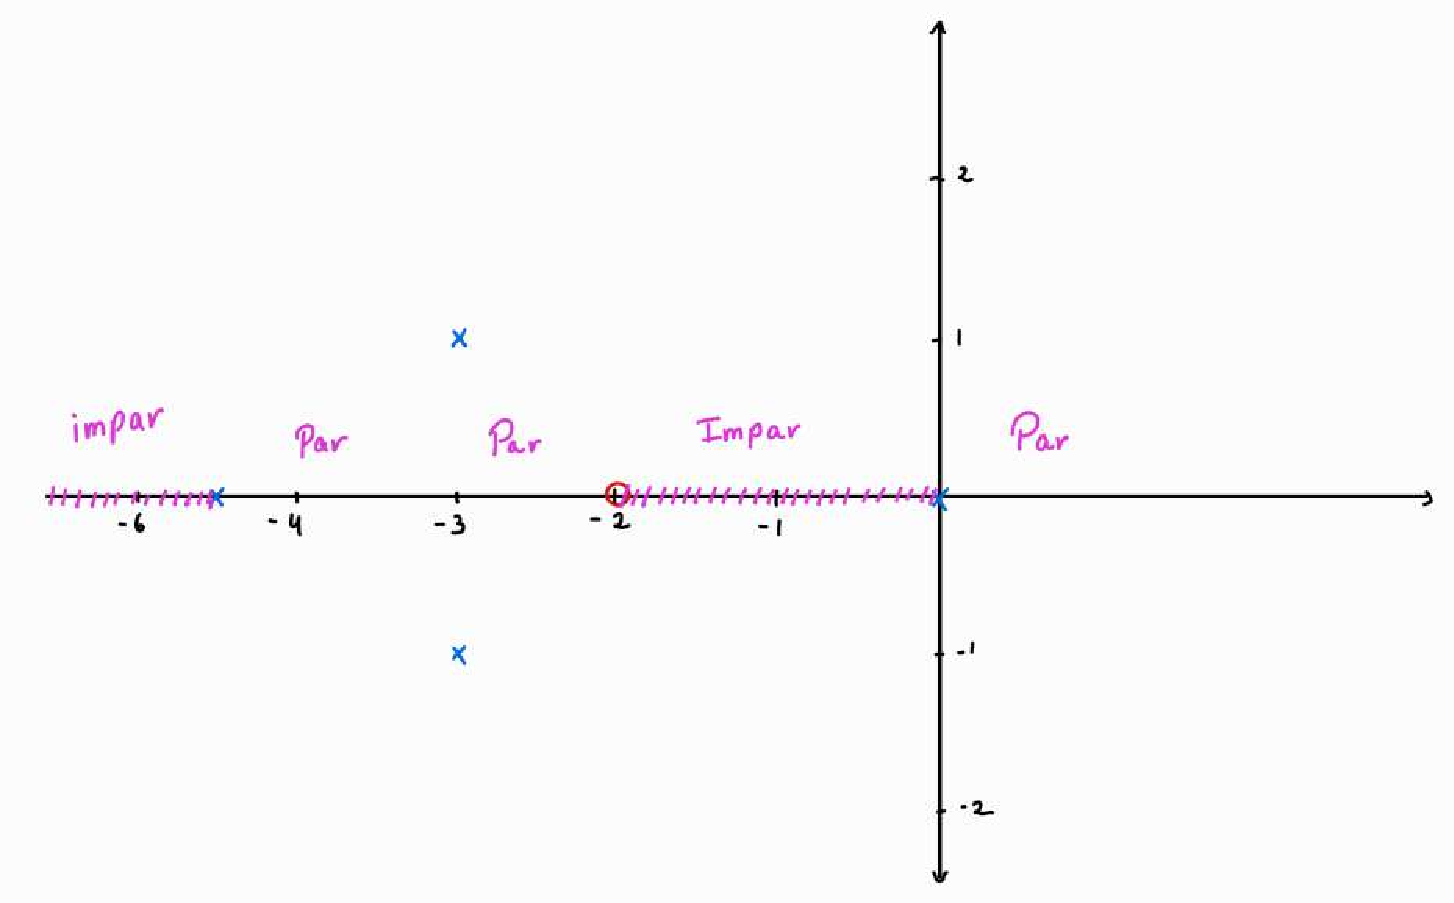
\includegraphics[width=0.6\textwidth]{Auxiliar_2_1}
    \end{figure}
\begin{enumerate}
    \item Establezca claramente el listado de hipótesis simplificatorias que permitan
    establecer un modelo matemático válido para este sistema. Indique las condiciones de borde y/o
    iniciales necesarias.
    \item Formule un modelo para el sistema en ecuaciones de estado.
    \item Caracterice completamente el modelo utilizando todos los puntos de vista descritos en clases.
    Clasifique todas las variables del sistema.
    \item Encuentre estado(s) cero, estado(s) de equilibrio y el estado tierra (de existir).
    \item Linealice el sistema en torno al (los) estado(s) de equilibrio encontrados.
\end{enumerate}
    %%%%%%%%%%%%%%%%%%%%%%%%%%%
\begin{solution}
\subsection*{Resolución 1.1}
Para poder formular un modelo del sistema, debemos primeramente considerar hipótesis simplificatorias que permitan simplificar el problema o poner límites sobre las distintas restricciones del mismo, por lo tanto:
\begin{itemize}
    \item Los parámetros \(V_{in},\,R,\,R_0,\,C\) son constantes del sistema.
    \item El circuito opera en régimen de \emph{parámetros concentrados}.
    \item Se desprecia la resistencia interna del voltímetro.
    \item No se consideran efectos parásitos ni ruidos.
    \item \dots
\end{itemize}
Por otra parte, por conocimiento de circuitos se sabe que la condición inicial necesaria para determinar el estado del sistema corresponde al voltaje inicial del condensador \(v_c(0)\).
\subsection*{Resolución 1.2}
Primero se aplica la Ley de Corrientes de Kirchhoff (LCK) en el nodo superior, con lo que se tiene \(I(t)=i_1(t)+i_2(t)\). Además, utilizando la Ley de Voltajes de Kirchhoff (LVK) en la malla izquierda se obtiene,
\begin{align}
V_{in}=RI+v_c \;=\; R i_1 + R i_2 + v_c .
\end{align}
Recordando la ecuación del condensador, \(i_C=C\,\dot v_c\), e identificando \(i_C=i_2\),
\begin{align}
V_{in}=R i_1 + RC\,\dot v_c + v_c .
\end{align}
En la rama de la derecha luego se tiene:
\begin{align}
v_c = R_0 i_1 + (\alpha\, i_2) i_1
    = R_0 i_1 + \alpha C \dot v_c\, i_1
    = \bigl(R_0 + \alpha C \dot v_c \bigr) i_1,
\end{align}
Despejando,
\begin{align}
i_1=\frac{v_c}{R_0+\alpha C \dot v_c}.
\end{align}
Sustituyendo la ecuación~(4) en la ecuación~(2) con el motivo de dejar todo en función de una única variable \(v_{c}\), luego se llega a:
\begin{align}
V_{in}= \frac{R\,v_c}{R_0+\alpha C \dot v_c} + RC\,\dot v_c + v_c .
\end{align}
Reordenando y desarrollando,
\begin{align}
R_0 V_{in}+ \alpha C V_{in}\dot v_c
= Rv_c + R_0 RC \dot v_c + \alpha RC^2 \dot v_c^{\,2} + R_0 v_c + \alpha C v_c \dot v_c ,
\end{align}
lo que lleva a la ecuación cuadrática en \(\dot v_c\):
\begin{align}
\alpha RC^2 \dot v_c^{\,2} + \bigl(R_0RC + \alpha C (v_c - V_{in})\bigr)\dot v_c
+ (R+R_0) v_c - R_0 V_{in} = 0.
\end{align}
Resolviendo para \(\dot v_c\),
\begin{align}
\dot v_c
= \frac{-\bigl(R_0RC + \alpha C (v_c - V_{in})\bigr) \pm \sqrt{S}}
       {2\alpha RC^2},
\end{align}
donde, por conveniencia,
\begin{align}
S
&= R_0^2 R^2 C^2
+ 2\alpha R_0 R C^2 (v_c - V_{in})
+ \alpha^2 C^2 (v_c - V_{in})^2 \nonumber\\
&\quad - 4\alpha R C^2 (R+R_0) v_c
+ 4 R_0 R C^2 V_{in}.
\end{align}
Alternativamente, dividiendo por \(RC\),
\begin{align}
\dot v_c
&= \frac{V_{in}-v_c}{2RC} - \frac{R_0}{2\alpha C} \nonumber\\
&\quad + \frac{1}{2\alpha C}\sqrt{
  R_0^2 + \frac{2\alpha R_0}{R}(v_c - V_{in})
  + \frac{\alpha^2}{R^2}(v_c - V_{in})^2
  - \frac{4\alpha (R+R_0)}{R} v_c + \frac{4R_0}{R}V_{in} } .
\end{align}
Con lo que se obtiene finalmente la ecuación diferencial que caracteriza el sistema, la cual es evidentemente \textbf{no lineal}.
\subsection*{Resolución 1.3}
Existen diversas características con las que podemos clasificar los modelos, algunas de estas son las siguientes:
\begin{center}
\begin{tabular}{|l|l|}
\hline
\textbf{Característica} & \textbf{Clasificación} \\
\hline
Origen & Fenómeno \emph{artificial} (sistema eléctrico construido) \\
\hline
Naturaleza & \emph{Determinístico} (no se consideran ruidos \(w(t)\) o \(v(t)\)) \\
\hline
Número de variables & \emph{Monovariable} (un estado) \\
\hline
Continuidad & \emph{Continuo} (aparece \(\dot v_c\)) \\
\hline
Comportamiento espacial & \emph{Parámetros concentrados} \\
\hline
Comportamiento temporal & \emph{Invariante en el tiempo} \\
\hline
Linealidad & \emph{No lineal} (por la dependencia racional en \(\dot v_c\)) \\
\hline
Realizabilidad & \emph{Causal y realizable} \\
\hline
\end{tabular}
\end{center}
Luego deberemos definir las variables del sistema, las cuales se pueden definir de la siguiente manera:
\begin{itemize}
    \item Estado: \(x(t)=v_c(t)\).
    \item Salida: \(y(t)=v_{out}(t)=v_c(t)=x(t)\).
    \item Entrada: \(u(t)=\alpha(t)\).
\end{itemize}
Es importante recordar que la elección de la salida es, por lo general, arbitraria a menos que se indique específicamente en el enunciado.
\subsection*{Resolución 1.4}
A continuación se analizan los diferentes estados del sistema:

\begin{itemize}
    \item \textbf{Estado cero.} Recordemos que un estado cero \(x_0 \in \Sigma\) de un sistema es tal que la salida \(y(t)\) cumple que \(y(t) = \overline{A}(x_0, 0) = 0\). En términos sencillos, es una condición inicial tal que, para entrada cero, la salida es cero. Como \(y=x\), el estado cero es
    \begin{align}
    x_0 = 0.
    \end{align}
    
    \item \textbf{Estado de equilibrio.} Recordemos que un estado de equilibrio \(x_e \in \Sigma\) es tal que \(x_e = \overline{B}(x_e, 0)\). Esto significa que bajo entrada cero, si el sistema está en estado de equilibrio entonces se quedará por siempre en este. Para encontrarlo, buscamos \(x_e\) tal que \(\dot x=0\). Evaluando la condición en la ecuación cuadrática se obtiene
    \begin{align}
    (R+R_0)\,x_e - R_0 V_{in}=0 \quad \Rightarrow \quad
    x_e = \frac{R_0}{R+R_0}\,V_{in}.
    \end{align}
    
    \item \textbf{Estado tierra.} Recordemos que un estado tierra \(x_t \in \Sigma\) de un sistema es tal que \(\forall x_0 \in \Sigma, \lim_{t \to \infty} \overline{B}(x_0, 0) = x_t\). El estado tierra es tal que, para toda condición inicial y con entrada cero, el sistema converge al estado tierra. Cuando el condensador está completamente cargado (tiempo suficientemente grande), no conduce corriente y el circuito equivale a un divisor de tensión. Por lo tanto,
    \begin{align}
    x_t = \frac{R_0}{R+R_0}\,V_{in}.
    \end{align}
\end{itemize}

\subsection*{Resolución 1.5}

El sistema linealizado alrededor del punto de operación \((\bar x,\bar u)\) viene dado por
\begin{align}
\dot{\tilde x} &= \left.\frac{\partial f}{\partial x}\right|_{\bar x,\bar u}\tilde x
               + \left.\frac{\partial f}{\partial u}\right|_{\bar x,\bar u}\tilde u, \\
\tilde y       &= \left.\frac{\partial g}{\partial x}\right|_{\bar x,\bar u}\tilde x
               + \left.\frac{\partial g}{\partial u}\right|_{\bar x,\bar u}\tilde u,
\end{align}
donde, a partir de la ecuación anterior, definimos
\begin{align}
f(v_c,\alpha) &= \frac{V_{in}-v_c}{2RC} - \frac{R_0}{2\alpha C}
+ \frac{1}{2\alpha C}\sqrt{
  R_0^2 + \frac{2\alpha R_0}{R}(v_c - V_{in})
  + \frac{\alpha^2}{R^2}(v_c - V_{in})^2
  - \frac{4\alpha (R+R_0)}{R} v_c + \frac{4R_0}{R}V_{in} }, \\
g(v_c,\alpha) &= v_c.
\end{align}

Derivadas parciales:
\begin{align}
\frac{\partial f}{\partial v_c}
&= -\frac{1}{2RC}
   - \frac{1}{4\alpha C \sqrt{S}}
      \left[\frac{2\alpha R_0}{R}
            + \frac{2\alpha^2}{R^2}(v_c-V_{in})
            - \frac{4\alpha (R+R_0)}{R}\right] \\
&= -\frac{1}{2RC}
   - \frac{1}{2RC\,\sqrt{S}}
      \left[R_0 + \frac{\alpha}{R}(v_c-V_{in}) - 2(R+R_0)\right],
\end{align}
donde
\begin{align}
S
= R_0^2 + \frac{2\alpha R_0}{R}(v_c - V_{in})
  + \frac{\alpha^2}{R^2}(v_c - V_{in})^2
  - \frac{4\alpha (R+R_0)}{R} v_c + \frac{4R_0}{R}V_{in}.
\end{align}
Análogamente,
\begin{align}
\frac{\partial f}{\partial \alpha}
&= \frac{R_0}{2\alpha^2 C}
   - \frac{1}{2\alpha^2 C}\sqrt{S}
   + \frac{1}{4C\sqrt{S}}
      \frac{\partial S}{\partial \alpha},
\end{align}
donde
\begin{align}
\frac{\partial S}{\partial \alpha}
= \frac{2 R_0}{R}(v_c - V_{in})
  + \frac{2\alpha}{R^2}(v_c - V_{in})^2
  - \frac{4 (R+R_0)}{R} v_c .
\end{align}
Para la salida,
\begin{align}
\frac{\partial g}{\partial v_c}=1, \qquad
\frac{\partial g}{\partial \alpha}=0.
\end{align}

Elegimos el punto de operación
\(
\bar x=\bar v = \dfrac{R_0}{R+R_0}V_{in},\;
\bar u=\bar\alpha=1
\).
Evaluando,
\begin{align}
A &= \left.\frac{\partial f}{\partial v_c}\right|_{\bar v,\,\bar\alpha}, \qquad
B = \left.\frac{\partial f}{\partial \alpha}\right|_{\bar v,\,\bar\alpha}, \qquad
C = 1,\qquad D=0.
\end{align}

Finalmente, el sistema linealizado en incrementos \(\tilde x:=x-\bar x\), \(\tilde u:=u-\bar u\) queda
\begin{align}
\dot{\tilde x} &= A\,\tilde x + B\,\tilde u, \\
\tilde y &= \tilde x.
\end{align}

\end{solution}


    %%%%%%%%%%%%%%%%%%%%%%%%%%%
    \question Considere el sistema linealizado del auxiliar anterior, modelado por la siguiente ecuación diferencial:
    \begin{equation}
        \ddot{\theta}(t) = \frac{g}{l} \theta(t) + \frac{1}{l} u(t)
    \end{equation}

    \begin{enumerate}
        \item Descomponer la salida como la suma de la respuesta a condiciones iniciales nulas y la respuesta a entrada nula en el dominio de Laplace.
        \item Obtener la función de transferencia del sistema y encontrar la respuesta al impulso con condiciones iniciales nulas en el dominio del tiempo.
        \item Obtener la respuesta a condiciones iniciales nulas en el dominio del tiempo, y expresar la respuesta para una entrada y condiciones iniciales arbitrarias.
        \item (Propuesta) Encontrar la salida cuando la entrada es un escalón unitario.
    \end{enumerate}

%%%%%%%%%%%%%%%%%%%%%%%%%%%

\begin{solution}
\subsection*{Resolución 2.1}
Para hacer la descomposición, trabajemos en el dominio de Laplace. Aplicando la transformada de Laplace sobre la EDO del sistema, considerando que:
\begin{equation}
L\left\{ \ddot{\theta}(t) \right\} = s^2 \Theta(s) - s \theta(0) - \dot{\theta}(0)
\end{equation}
tenemos
\begin{equation}
s^2 \Theta(s) - s \theta(0) - \dot{\theta}(0) = \frac{g}{l} \Theta(s) + \frac{1}{l} U(s)
\end{equation}
Reordenando para despejar el término de la salida, tenemos
\begin{equation}
\Theta(s) = \frac{s\theta(0) + \dot{\theta}(0)}{s^2 - \frac{g}{l}} + \frac{1}{s^2 - \frac{g}{l}} \frac{1}{l} U(s)
\end{equation}
donde podemos ver que la salida \(\Theta(s)\) está escrita como la suma de dos términos. El primero de ellos corresponde a
\begin{equation}
\Theta_0(s) = \frac{s \theta(0) + \dot{\theta}(0)}{s^2 - \frac{g}{l}},
\end{equation}
el cual está asociado a la salida cuando se tienen condiciones iniciales arbitrarias pero entrada nula, y corresponde a la RENC del sistema (Respuesta a Entrada Nula o Cero). El segundo término es
\begin{equation}
\Theta_s(s) = \frac{1}{l} \frac{1}{s^2 - \frac{g}{l}} U(s),
\end{equation}
y corresponde a la salida en el caso donde utilizamos condiciones iniciales nulas, pero una entrada arbitraria, y es denominada RESC (Respuesta a Estado Cero). Así, podemos ver que
\begin{equation}
\Theta(s) = \Theta_0(s) + \Theta_s(s),
\end{equation}
por lo que la salida se puede escribir como la suma de RENC y RESC.

\subsection*{Resolución 2.2}
La noción de función de transferencia está ligada estrechamente con la RESC, ya que para obtener la función de transferencia, asumimos condiciones iniciales nulas y una entrada arbitraria. Haciendo estos supuestos, tenemos:
\begin{equation}
\Theta(s) = \frac{1}{l} \frac{1}{s^2 - \frac{g}{l}} U(s)
\end{equation}
Luego, la función de transferencia \(H(s)\) del sistema se define como:
\begin{equation}
H(s) = \frac{\Theta(s)}{U(s)},
\end{equation}
donde es importante notar que utilizamos la RESC para definirla, dado que como se mencionó anteriormente, asumimos condiciones iniciales nulas, por lo que podemos ver que se tiene
\begin{equation}
H(s) = \frac{1}{l} \frac{1}{s^2 - \frac{g}{l}}.
\end{equation}
Definiendo \(\omega_0 := \sqrt{\frac{g}{l}}\), tenemos
\begin{equation}
H(s) = \frac{1}{l} \frac{1}{(s + \omega_0)(s - \omega_0)}.
\end{equation}

\subsection*{Resolución 2.3}
Luego, para obtener la respuesta al impulso en el dominio del tiempo \(h(t)\), debemos considerar que \(L\left\{ \delta(t) \right\} = 1\), por lo que si la entrada es un impulso \(u(t) = \delta(t)\), entonces \(U(s) = 1\). Así, dado que la función de transferencia es
\begin{equation}
H(s) = \frac{\Theta(s)}{U(s)},
\end{equation}
si \(U(s) = 1\), podemos ver que \(H(s)\) correspondería a la respuesta al impulso en el dominio de Laplace, por lo que para obtenerla en el dominio del tiempo, bastaría aplicar la transformada inversa a la función de transferencia, tal que:
\begin{equation}
h(t) = L^{-1}\{H(s)\}.
\end{equation}

\subsection*{Resolución 2.4}
Para hacerlo, debemos tener en mente que:
\begin{equation}
L\left\{ e^{\alpha t} \right\} = \frac{1}{s - \alpha}.
\end{equation}
Por otra parte, sabemos que:
\begin{equation}
H(s) = \frac{1}{l} \frac{1}{(s + \omega_0)(s - \omega_0)},
\end{equation}
por lo que podemos aplicar una descomposición en fracciones parciales para expresar \(H(s)\) como:
\begin{equation}
H(s) = \frac{\alpha}{s + \omega_0} + \frac{\beta}{s - \omega_0}.
\end{equation}
Luego podríamos aplicar la inversa de forma sencilla. Para esto, encontremos \(\alpha\) y \(\beta\). Si comenzamos intentando encontrar \(\alpha\), notemos que en la ecuación (16) podemos multiplicar por \(s + \omega_0\) para obtener:
\begin{equation}
H(s)(s + \omega_0) = \alpha + \frac{\beta}{s - \omega_0} (s + \omega_0),
\end{equation}
donde podemos ver que el término \(\frac{\beta}{s - \omega_0}\) no nos permite obtener \(\alpha\) directamente. Sin embargo, notemos que podemos evaluar esta expresión en \(s = -\omega_0\), de donde tendríamos:
\begin{equation}
H(s) (s + \omega_0)\Big|_{s=-\omega_0} = \alpha + \frac{\beta}{s - \omega_0} (s + \omega_0)\Big|_{s=-\omega_0} = 0.
\end{equation}
Por lo que tenemos:
\begin{equation}
\alpha = H(s) (s + \omega_0)\Big|_{s=-\omega_0}.
\end{equation}
Equivalentemente, se puede realizar un desarrollo análogo para obtener \(\beta\), de donde se obtiene:
\begin{equation}
\beta = H(s) (s - \omega_0)\Big|_{s=\omega_0}.
\end{equation}
Utilizando estas expresiones para calcular los coeficientes, tenemos:
\begin{equation}
\alpha = H(s) (s + \omega_0)\Big|_{s=-\omega_0} = \frac{1}{l} \frac{1}{(s + \omega_0)(s - \omega_0)} (s + \omega_0)\Big|_{s=-\omega_0} = \frac{1}{l} \frac{1}{s - \omega_0}\Big|_{s=-\omega_0} = -\frac{1}{2 \omega_0 l}.
\end{equation}
Para \(\beta\), tenemos:
\begin{equation}
\beta = H(s) (s - \omega_0)\Big|_{s=\omega_0} = \frac{1}{l} \frac{1}{(s + \omega_0)(s - \omega_0)} (s - \omega_0)\Big|_{s=\omega_0} = \frac{1}{l} \frac{1}{s + \omega_0}\Big|_{s=\omega_0} = \frac{1}{2 \omega_0 l}.
\end{equation}
Luego, juntando ambos términos, podemos descomponer \(H(s)\) como:
\begin{equation}
H(s) = \frac{1}{2 \omega_0 l} \left( \frac{1}{s - \omega_0} - \frac{1}{s + \omega_0} \right).
\end{equation}
Con esta descomposición, podemos aplicar la inversa para obtener \(h(t)\), de modo que:
\begin{equation}
h(t) = L^{-1}\left\{ \frac{1}{2 \omega_0 l} \left( \frac{1}{s - \omega_0} - \frac{1}{s + \omega_0} \right) \right\}.
\end{equation}
Finalmente, recordemos que, como vimos anteriormente, tenemos:
\begin{equation}
h(t) = \frac{1}{2 \omega_0 l} \left( e^{\omega_0 t} - e^{-\omega_0 t} \right).
\end{equation}

\end{solution}
\end{questions}
\end{document}